\subsection{Ranking within a fixed opacity band}\label{sec:bridge}
An earlier matched experiment held the opacity core, candidate band, source and count fixed and changed the ordering within the band. The comparators used the opacity--scale product in Eq.~\eqref{eq:legacy-score}, one frozen random order per source, or a feedback-based protected ordering (H). The first two controls isolate the contribution of the ranking within the same band. H also changes the calibration procedure.
\begin{table}[htbp]
\centering
\caption{Effect of changing the ranking within the protected band at 25\% retention. Each entry is the mean paired difference in cold PSNR (P minus comparator, dB) across three sources. Positive values favor P.}\label{tab:scorebridge}
\begin{tabular}{lrrr}
\toprule
Scene & Opacity--scale & Random order & Feedback (H) \\
\midrule
Chicken & +3.0496 & +2.6040 & -0.0418 \\
Cut roasted beef & +2.1925 & +2.4405 & -0.0331 \\
Sear steak & +2.1149 & +2.2713 & -0.0305 \\
Basin & +0.0133 & +0.0750 & +0.0003 \\
\bottomrule
\end{tabular}
\end{table}

P outperformed the opacity--scale product and the fixed random order on all twelve sources. Feedback yielded higher PSNR than P on eleven. The latter improvement adds an offline cost: on Chicken, Cut roasted beef and Sear steak, the median selection time over three independent processes was 3.22--3.37 times as long for H as for P. Including loading and saving reduced the ratio to 1.49--1.57. These measurements compare the preparation cost of P and H only. Peak allocated memory during selection was higher for P.\par

\subsection{What remains visible at one quarter of the points}\label{sec:visual}
Figure~\ref{fig:visual} compares the same test view across the observation, the complete source, and three cold subsets. In all three frames, reranking recovers part of the quality lost under opacity truncation. We also compared the central $192\times144$ pixels against ground truth for all nine archived example views (three per scene, seed 0). In the 8-bit images, full-source crop PSNR exceeded cold C crop PSNR in all nine pairs, by 0.047--0.757~dB. The crop measurements quantify local reconstruction error, whereas the labels in the figure describe the entire frame.
\begin{figure}[htbp]
\centering
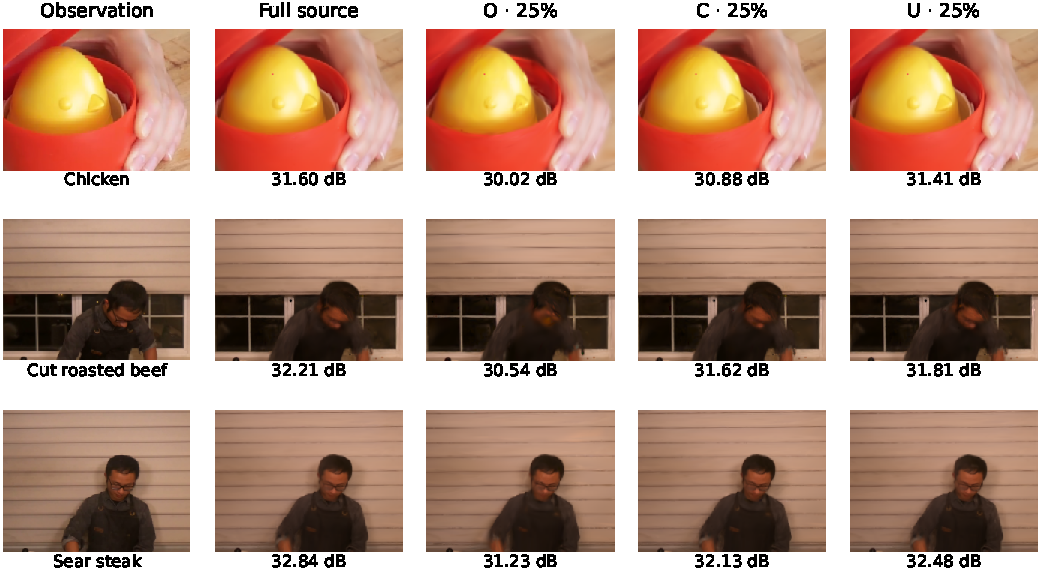
\includegraphics[width=\linewidth]{qualitative.pdf}
\caption{Matched central crops at 25\% retention. Each row uses seed 0 and the middle of three archived example views (source indices 165, 150, and 150, respectively). Each crop spans the central $192\times144$ native pixels. Values below the renderings give PSNR for the entire corresponding frame. The full-source column uses all points from the same source as the three subsets.}\label{fig:visual}
\end{figure}

For Press, a separate historical experiment on the protected-core order P contains 487 paired $240\times135$ test frames per seed across three seeds. At 25\% retention the mean full-minus-P PSNR gap is 0.018~dB, while the largest individual frame gap is 0.353~dB. These frame averages characterize the archived Press runs. The original figure used a separate rendering record.
